
%%%%%%%%%%%%%%%%%%%%%%%%%%%%%%%%%%%%%%%%%
% Short Sectioned Assignment LaTeX Template Version 1.0 (5/5/12)
% This template has been downloaded from: http://www.LaTeXTemplates.com
% Original author:  Frits Wenneker (http://www.howtotex.com)
% License: CC BY-NC-SA 3.0 (http://creativecommons.org/licenses/by-nc-sa/3.0/)
%%%%%%%%%%%%%%%%%%%%%%%%%%%%%%%%%%%%%%%%%

% \documentclass[paper=a4, fontsize=11pt]{scrartcl} % A4 paper and 11pt font size
\documentclass[11pt, a4paper, oneside]{book}
\usepackage[T1]{fontenc} % Use 8-bit encoding that has 256 glyphs
\usepackage[utf8]{inputenc}
\usepackage{fourier} % Use the Adobe Utopia font for the document - comment this line to return to the LaTeX default
\usepackage{listings} % para insertar código con formato similar al editor
\usepackage[spanish, es-tabla]{babel} % Selecciona el español para palabras introducidas automáticamente, p.ej. "septiembre" en la fecha y especifica que se use la palabra Tabla en vez de Cuadro
\usepackage{url} % ,href} %para incluir URLs e hipervínculos dentro del texto (aunque hay que instalar href)
\usepackage{graphics,graphicx, float} %para incluir imágenes y colocarlas
\usepackage[gen]{eurosym} %para incluir el símbolo del euro
\usepackage{cite} %para incluir citas del archivo <nombre>.bib
\usepackage{enumerate}
\usepackage{hyperref}
\usepackage{graphicx}
\usepackage{tabularx}
\usepackage{booktabs}
\usepackage{indentfirst}
\usepackage[table,xcdraw]{xcolor}
\hypersetup{
	colorlinks=true,	% false: boxed links; true: colored links
	linkcolor=black,	% color of internal links
	urlcolor=cyan		% color of external links
}
\renewcommand{\familydefault}{\sfdefault}
\usepackage{fancyhdr} % Custom headers and footers
\pagestyle{fancyplain} % Makes all pages in the document conform to the custom headers and footers
\fancyhead[L]{} % Empty left header
\fancyhead[C]{} % Empty center header
\fancyhead[R]{Cecilia Merelo Molina} % My name
\fancyfoot[L]{} % Empty left footer
\fancyfoot[C]{} % Empty center footer
\fancyfoot[R]{\thepage} % Page numbering for right footer
%\renewcommand{\headrulewidth}{0pt} % Remove header underlines
\renewcommand{\footrulewidth}{0pt} % Remove footer underlines
\setlength{\headheight}{13.6pt} % Customize the height of the header

\usepackage{titlesec, blindtext, color}
\definecolor{gray75}{gray}{0.75}
\newcommand{\hsp}{\hspace{20pt}}
\titleformat{\chapter}[hang]{\Huge\bfseries}{\thechapter\hsp\textcolor{gray75}{|}\hsp}{0pt}{\Huge\bfseries}
\setcounter{secnumdepth}{4}
\usepackage[Lenny]{fncychap}

\begin{document}
	% Plantilla portada UGR
	\input{portada/portada}

	% Plantilla prefacio UGR
	\thispagestyle{empty}

\begin{center}
{\large\bfseries Algoritmos Basados En Población Con Diversidad Mejorada \\ Algoritmo basado en Un Mundo Feliz de Aldous Huxley }\\
\end{center}
\begin{center}
Cecilia Merelo Molina\\
\end{center}

%\vspace{0.7cm}

\vspace{0.5cm}
\noindent{\textbf{Palabras clave}: \textit{software libre}
\vspace{0.7cm}

\noindent{\textbf{Resumen}\\
	

\cleardoublepage

\begin{center}
	{\large\bfseries Algorithm Based In a Diversity-Improved Population}\\
\end{center}
\begin{center}
	Cecilia Merelo Molina\\
\end{center}
\vspace{0.5cm}
\noindent{\textbf{Keywords}: \textit{open source}, \textit{floss}
\vspace{0.7cm}

\noindent{\textbf{Abstract}\\

At the beginning of this year I read "A brave new world" by Aldous Huxley. This novel describes a dystopia, 
which anticipates the development of breeding technology, and how this technology creates the perfect human race; that is, essentially a population based optimization algorithm,of which a well known kind are evolutionary algorithms. This book kind of describes the process for making the “perfect human”, so this similitude is what we will try to develop in this paper. 
The goal is to develop a genetic algorithm based on the fecundation process of the book and compare it to other algorithms to see how it behaves, investigating how the division in castes affects the diversity in the population.

\cleardoublepage

\thispagestyle{empty}

\noindent\rule[-1ex]{\textwidth}{2pt}\\[4.5ex]

D. \textbf{Tutora/e(s)}, Profesor(a) del ...

\vspace{0.5cm}

\textbf{Informo:}

\vspace{0.5cm}

Que el presente trabajo, titulado \textit{\textbf{Chief}},
ha sido realizado bajo mi supervisión por \textbf{Estudiante}, y autorizo la defensa de dicho trabajo ante el tribunal
que corresponda.

\vspace{0.5cm}

Y para que conste, expiden y firman el presente informe en Granada a Junio de 2018.

\vspace{1cm}

\textbf{El/la director(a)/es: }

\vspace{5cm}

\noindent \textbf{(nombre completo tutor/a/es)}

\chapter*{Agradecimientos}






	% Índice de contenidos
	\newpage
	\tableofcontents

	% Índice de imágenes y tablas
	\newpage
	\listoffigures

	% Si hay suficientes se incluirá dicho índice
	\listoftables 
	\newpage

	% Introducción 
	\input{secciones/01_introduccion}

	% Descripción del problema y hasta donde se llega
	\chapter{Descripción del problema y caracterización de la solución}

En este capítulo se describe el problema cuya solución se quiere abordar en este trabajo. Primero se analiza la naturaleza del algoritmo que
se quiere implementar, luego se describe la metaheurística que se va a desarrollar, para acabar con los casos de uso que se han ido
implementando hasta conseguir la funcionalidad completa.

\section{Descripción}

En 2019, para la asignatura de metaheurísticas de la Universidad de Granada \cite{merelo_molina_2021} se propuso inventar una 
metaheurística. En ese momento acababa de leer el libro ``Un Mundo feliz`` de Aldous Huxley \cite{un_mundo_feliz_libro}, así que
decidí adaptar el proceso de optimización de la población humana que describe el libro a un algoritmo evolutivo. A lo largo del
desarrollo se me presentaron varios retos. El primero fue el lenguaje escogido; lo desarrollé en Python, un lenguaje caracterizado
por su fácil sintaxis pero su deficiencia de velocidad. Cada ejecución del problema llevaba horas, por lo que se hacía muy difícil
de ejecutar y analizar. El segundo fue la optimización de los parámetros; el algoritmo quedaba estancado en óptimos locales.
Estos problemas son los que se quieren abordar en el desarrollo de este trabajo.

Como se ha mencionado en la sección anterior, y relacionado con los objetivos de desarrollar una herramienta de altas prestaciones,
se quiere desarrollar una metaheurística inspirada por un libro. Pero no solo interesa
el poder adaptar el proceso descrito en el libro a una metaheurística. También se busca que la metaheurística pueda ser
usada fácilmente por la comunidad, que su implementación sea extensible y mantenible, y además fácil de analizar, para completar el objetivo
desarrollo mediante metodología ágil. Para conseguirlo se desarrollará una biblioteca que sea adaptable al problema a resolver, donde los parámetros iniciales sean indicados por la persona que use el algoritmo; parámetros como la función de fitness,
tamaño de la población inicial, dimensión del cromosoma y rango de búsqueda

\section{Naturaleza del algoritmo}

Como se ha mencionado, el algoritmo está basado en el proceso de optimización de la población humana que describe el libro, por tanto,
estamos hablando de un algoritmo basado en la evolución de una población, así que seguirá
la estructura de los algoritmos evolutivos, más en concreto, un \emph{algoritmo genético}. Se trata de un algoritmo 
genético ya que es un algoritmo de optimización de búsqueda inspirado en los procesos de Evolución Natural y
Evolución Genética.

Siguiendo la definición dada por Goldberg \cite{goldberg89}, "los Algoritmos Genéticos son algoritmos de búsqueda
basados en la mecánica de selección natural. Combinan la supervivencia del más apto entre estructuras de secuencias con un intercambio de 
información estructurado, aunque aleatorizado, para construir así un algoritmo de búsqueda que tenga algo de las genialidades de las 
búsquedas humanas". En resumen, estos algoritmos reflejan el proceso de la selección natural. Forman parte del grupo de 
los \emph{algoritmos evolutivos}. El proceso está compuesto de 4 componentes principales:

\begin{itemize}
    \item Creación de la población inicial: el proceso comienza con un conjunto de individuos llamado \emph{Población}. Cada individuo
    representa una solución del problema a resolver. Cada individuo se caracteriza por una serie de parámetros llamados
    \emph{genes}. Los genes se unen para formar un \emph{Cromosoma}. Estos se crean en la primera generación. La población del 
    resto de generaciones serán evoluciones de esta población inicial.
    \item Selección: la idea de la fase de selección es seleccionar los individuos más adecuados para que pasen sus
    genes a las siguientes generaciones. Los individuos con mejor valor de fitness son los que tienen más posibilidades
    de ser seleccionados para la reproducción.
    \item Cruce: produce un nuevo individuo por cada pareja de padres, seleccionando de uno de ellos un segmento
    continuo de características y copiándolo en la descendencia. Los genes que quedan por asignar en la descendencia
    combinan de manera uniforme características de los dos padres.
    \item Mutación: en los hijos, algunos de los genes pueden ser sometidos a mutación, es decir, alguno de sus genes
    serán cambiados.
\end{itemize}

Además de las fases, también se debe definir una \emph{condición de parada} y una \emph{función de fitness}. La
condición de parada sirve para que el algoritmo finalice si la población converge, es decir, si no produce hijos 
que sean diferentes con respecto a las generaciones anteriores, o si alcanza la solución. La función de fitness
determina cómo de adecuado es un individuo, esto es, la probabilidad de que un individuo sea seleccionado para
la reproducción depende de este valor. Por tanto, para alcanzar la solución a un problema se parte de un conjunto 
inicial de individuos, llamado \textit{población inicial}, generado de manera aleatoria. Cada uno de estos 
individuos representa una posible solución al problema. Estos individuos van pasando por los diferentes operadores y 
evolucionando en cada generación.

En el caso del algoritmo propuesto en este trabajo (\emph{Algoritmo Feliz}) la población evolucionará siguiendo un proceso 
inspirado por los distintos mecanismos descritos en el libro de Aldous Huxley. El proceso propuesto se describe con mayor detalle
en la sección \ref{sect: description}. Al usar como guía los procesos descritos en el libro quiere decir que se está desarrollando 
una \textit{metaheurística}. Las  metaheurísticas son métodos de alto nivel, independientes del problema, que proporcionan una serie de guías o
estrategias para desarrollar algoritmos de optimización heurísticos \cite{metaheuristics_def}. Muchas metaheurísticas
están inspiradas en la naturaleza \cite{Molina2020ComprehensiveTO}. Por ejemplo, la optimización basada en colonias de
hormigas que imita la manera en la que las hormigas se comportan cuando viajan a una fuente de comida, y cómo se 
comunican unas con otras a través de feromonas. 

Normalmente las metaheurísticas se usan en problemas de optimización por varias razones:
\begin{itemize}
    \item Encuentran maneras de ir de una solución a otra mejor sin tener por qué considerar todas las posibles combinaciones. 
    \item Pueden evitar quedarse estancadas en mínimos locales porque usan aleatoriedad.
\end{itemize}

En conclusión, se va a desarrollar una metaheurística basada en el proceso de fecundación y la división en castas descrita en el 
libro de A. Huxley, llamada ``Algoritmo Feliz`` o \emph{AF}.

\section{Descripción de la metaheurística desarrollada} \label{sect: description}

El libro describe cómo se alcanza esta raza humana perfecta mediante una ``cadena de montaje``, con varias fases. Esto lo 
reflejaremos mediante un algoritmo evolutivo generacional con los operadores de selección, cruce, mutación y reemplazamiento. 
El proceso comienza en la \textbf{\textit{Sala de Fecundación}}; aquí se crean los óvulos y se fecundan. Una vez \textit{fecundados}
los óvulos pasan a las incubadoras, donde se decide la \textit{casta} a la que pertenecerá cada individuo. Huxley describe 
como a los Alfas y los Betas se les suministra una gran cantidad de nutrientes y hormonas durante la incubación. Mientras que las
castas bajas, Gamma, Delta y Epsilon son privadas de estos elementos necesarios para el desarrollo. Para imitar esta
 ``falta de nutrientes``, en el algoritmo a desarrollar privaremos a las castas bajas de operadores, solo mutarán. Con esto
 pretendo avanzar el objetivo de mantener la diversidad alta durante toda la ejecución del algoritmo. 
 Las castas se implementarán de la siguiente manera: 

\begin{itemize}
    \item \textbf{Alfas}:
        \begin{itemize}
            \item Libro: son los más inteligentes, a este grupo pertenece la élite. Tienen responsabilidades y son
            los que tienen la capacidad de tomar decisiones.
            \item Implementación: se reproducirán solo entre ellos, pasarán por todos los operadores del algoritmo.
        \end{itemize}
    \item \textbf{Betas}: 
        \begin{itemize}
            \item Libro: son menos inteligentes que los anteriores y su función principal se reduce a tareas
            administrativas.
            \item  Implementación: el cruce sólo se realiza con individuos Alpha.
        \end{itemize}
    \item \textbf{Gammas}: 
        \begin{itemize}
            \item Libro: son los empleados subalternos, cuyas tareas requieren de habilidad. Son expertos en tareas repetitivas
            \item Implementación: los individuos de esta casta solo tendrán mutación por búsqueda local.
        \end{itemize}
    \item \textbf{Castas Bajas}: sólo tendrán el operador de mutación por segmento fijo, sin búsqueda local. A este sector pertenecen:
        \begin{itemize}
            \item \textbf{Deltas}:a este grupo pertenecen los empleados de los anteriores.
            \item \textbf{Epsilones}: es la casta inferior, a ella pertenecen los empleados para trabajos arduos.
        \end{itemize}
\end{itemize}

Con esta estructura en mente la metaheurística se divide en las siguientes fases:

\begin{itemize}
    \item \textbf{Sala de Fecundación}: los individuos son creados de manera totalmente aleatoria. Tantos individuos
    como indique un parámetro \textit{I}.
    \item \textbf{Sala de incubación}: en esta fase realizamos la división en castas. Se hará basándonos en el valor de
    la función objetivo del individuo. Además cada casta tendrá un porcentaje diferente de la población. Ya que en el libro
    describe que las castas bajas se reproducen mediante el proceso de \textit{Bokanovsky}, donde un embrión, que normalmente 
    se desarrolla hasta convertirse en un adulto, se convierte en 96 gemelos idénticos. Esto en el algoritmo se reflejará 
    en el tamaño de la población, que descenderá cuanto más alta sea la casta.    
    \item \textbf{Evolución de las castas}: cada casta seguirá un proceso de evolución diferente como ya se 
    ha mencionado.
\end{itemize}

No se trata de castas estáticas, se generan al principio de cada generación. Imaginemos que tenemos una población de 10 individuos, cada 
uno con un valor de fitness. En la primera iteración se dividirá esta población atendiendo a este valor de fitness. Posteriormente,
cada individuo seguirá el proceso de evolución correspondiente a su casta. Al final de la generación se juntan todos los cromosomas,
independientemente de su casta, ya habrá evolucionado su valor con respecto al resto de los individuos de la
población. La siguiente generación comienza dividiendo en castas los cromosomas que han evolucionado en la anterior.

\section{Naturaleza del software} \label{sect:no-funcionales}

Alineados con los objetivos del TFG \ref{sect:goals}, los requisitos no funcionales de este proyecto son:

\begin{itemize}
    \item Desarrollo \emph{future-proof}: toda la funcionalidad debe ser testeada, de esta manera, en el futuro,
    cuando se hagan cambios se sabrá si la nueva funcionalidad rompe lo escrito hasta el momento o no. Esto
    también favorece que gente ajena al proyecto se vea más segura a participar en él. Además esto incrementa
    la mantenibilidad del código, ya que los tests ayudan a que siempre esté claro lo que hace cada método
    del código.
    \item Evitar la repetición de código, esto favorece a que el código sea más fácil de mantener.
    \item Desarrollo ágil: desarrollar la mínima cantidad de código que cubra la funcionalidad.
\end{itemize}

Este proyecto es software libre, y está liberado con la licencia \cite{gplv3}. El producto final de este proyecto será una
biblioteca que estará disponible Github \cite{project_repository}. Esto ayuda a la reproducibilidad de la ciencia y 
adicionalmente es parte de desarrollo ágil, ya que cualquier persona puede añadir tareas y marcarle la prioridad. Esto va
también en línea con la ciencia abierta. El concepto de “ciencia abierta” es la difusión del conocimiento científico 
lo más amplia posible, libre para todas y todos, accesible en línea y reutilizable


	% Estado del arte
	% 	1. Crítica al estado del arte
	% 	2. Propuesta
	\input{secciones/03_estado_del_arte}
	
	\input{secciones/04_planificacion}

	% Desarrollo bajo sprints: 
	% 	1. Permitir registros y login de usuarios
	% 	2. Desarrollo del sistema de incidencias
	% 	3. Desarrollo del sistema de denuncias administrativas y accidentes
	% 	4. Desarrollo del sistema de croquis
	%   5. Instalación de la aplicación de manera automática
	\chapter{Implementación}
En esta sección se va a describir la implementación, basada en los requisitos mencionados.

\section{Lenguaje de programación}

Una de las formas de conseguir altas prestaciones, para alcanzar el objetivo 2, es escoger el lenguaje adecuado. Por ello se ha elegido
un lenguaje que hace poco entró en el \"Petaflop Club\", el cual incluye aquellos lenguajes que superan 1 petaflop/segundo como rendimiento pico. Se trata
de Julia \cite{julia}, un lenguaje de programación multiparadigma de tipado dinámico. Orientado a la computación técnica y
científica, el objetivo de sus creadores fue el de combinar lo mejor de otros lenguajes, es decir, conseguir un “todo en uno”, lo que se traduce en:
la velocidad de C, la usabilidad de Python, el dinamismo de Ruby, la destreza matemática de MatLab, y las estadísticas de R \cite{julia_goals}.

\section{Metodología de desarrollo}

Un requisito fundamental a la hora de implementar es usar una metodología que garantice la evolución del código. Por eso la implementación 
del software se ha dividido en tareas, siguiendo la metodología ágil Kanban. Se divide pues el proyecto en tareas pequeñas que aporten valor al producto 
final, de esta forma que puedes probar cada tarea a medida que la vas acabando. Al final del desarrollo estás segura de que todas las piezas funcionan
correctamente.

Otro requisito es desarrollar un algoritmo que sea mantenible. Por tanto, a la hora del desarrollo se priorizarán conceptos 
como arquitectura limpia \cite{cleanArquitecture2017} y la limpieza del código \cite{cleanCode2008}, así como el desarrollo basado en tests. De esta manera, se asegura
que el algoritmo está asentado sobre una base firme. Asimismo, gracias al desarrollo basado en tests, para cada cambio que se haga
se sabrá si se ha roto lo que estaba escrito hasta el momento.  Usar estándares va en línea con el objetivo de aplicar el desarrollo ágil a la ciencia.

\section{Estructuras de datos}

Las entidades que se han utilizado para estructura la información son:
\begin{itemize}
    \item Para tener bien definidos los datos de entrada se ha creado una entidad que contiene todos los parámetros de
    configuración del algoritmo. Se trata de una estructura inmutable, luego estos parámetros no cambiarán a lo largo de todo el
    algoritmo.
    \item Para unificar todos los datos que necesita el algoritmo, se ha definido una estructura inmutable. Una vez
    rellenada esta entidad, el algoritmo tiene todos los datos necesarios para comenzar la ejecución.
    \item Definir la casta como una entidad abstracta. Julia usa el \emph{dispatch} múltiple como paradigma, 
    lo que va a ser muy útil a la hora de definir los operadores, como se verá más adelante. Teniendo la casta 
    como tipo abstracto podremos definir métodos que acepten cualquier tipo de casta.

    \item Julia es un lenguaje de tipado dinámico, pero tiene alguna de las ventajas del tipado estático, haciendo posible indicar
    los tipos de algunos valores. Además, para poder hacer buen uso de este paradigma se han definido las castas como tipos distintos, por ejemplo, para
    la casta alfa:

    \begin{lstlisting}[
        basicstyle=\small
    ]
        @with_kw struct ALPHA <: Caste
            name::String = "ALPHA"
        end
    \end{lstlisting}

    El decorador \lstinline{with_kw} de la biblioteca \emph{Parameters.jl}, para poder añadir parámetros por defecto a una entidad. Las castas se han definido 
    como tipos inmutables, ya que en ningún momento se va a cambiar el nombre propio de la casta.
\end{itemize}

\section{Implementación de los casos de uso}

En esta sección se va a describir las decisiones técnicas que se han tomado para desarrollar los casos de uso \ref{sect:use_cases}

\begin{itemize}
    \item \textbf{Sistema de entrada de la biblioteca} \ref{it:sist_entrada}: usar el formato JSON para definir los parámetros
    del algoritmo. Un ejemplo de fichero sería el siguiente:
    \begin{lstlisting}[
        basicstyle=\small
    ]
        {
            "CHROMOSOME_SIZE": 2,
            "POPULATION_SIZE": 100,
            "MAX_GENERATIONS": 15,
            "POPULATION_PERCENTAGE": {
                "ALPHA": 10,
                "BETA": 20,
                "GAMMA": 20,
                "DELTA": 20,
                "EPSILON": 30
            },
            "MUTATION_RATE": {
                "ALPHA": 10,
                "BETA": 10,
                "GAMMA": 10,
                "DELTA": 10,
                "EPSILON": 10
            }
        }
    \end{lstlisting}

    Cualquiera de estos parámetros se puede cambiar. Esto se convertirá en una entidad inmutable que servirá como 
    entrada al algoritmo.

    \item \textbf{Función de fitness \cite{project_repository_8}}: se han usado las funciones que pertenecen al \emph{benchmark}
    \emph{ Black-box Optimization Benchmarking (BBOB)} \cite{bbob_definition}. Este \emph{benchmark} define funciones que se suelen 
    usar como referencia en el campo de las metaheurísticas. En Julia están implementadas en la biblioteca 
    \emph{BlackBoxOptimizationBenchmarking.jl} \cite{bbob_jl}.

    \item \textbf{Operadores de selección, cruce y mutación} [\ref{it:selection_operator}, \ref{it:crossover_operator}, \ref{it:mutation_operator}]:
    Se ha usado el \emph{dispatch} múltiple para definir operadores que se adecúen en cada casta. Por ejemplo, para el caso del
    operador de selección se han definido 3 tipos de parámetros de entrada:

    \begin{lstlisting}[
        basicstyle=\small
    ]
        selector_operator(
            caste::ALPHA, 
            caste_population
        )
        selector_operator(
            caste::BETA, 
            caste_population, 
            alpha_reproduction_pool
        )
        selector_operator(
            caste, 
            caste_population
        )
    \end{lstlisting}
    
    Para muestrear la población se ha usado la biblioteca \emph{StatsBase.jl}. Se ha elegido esta librería porque
    tiene un gran número de contribuidores y se actualiza continuamente.
\end{itemize}

\section{Implementación del cálculo de la diversidad}

Uno de los objetivos del TFG es mejorar la diversidad en problemas de optimización mediante la división de la población en castas.
Para calcularla se han usado como métricas la entropía y la distancia de edición; la decisión de usar estas medidas

está definida en secciones posteriores. Para calcular la entropía en Julia hay varias librerías disponibles:

\begin{itemize}
    \item \emph{Entropy.jl} \cite{entropy_jl}: este paquete contiene funcionalidad para ejecutar estimaciones de la entropía. No se ha usado porque,
    aparte de no tener nada de documentación, la última vez que se actualizó fue hace 8 años, por tanto contiene
    sintaxis antigua que no compilará con las nuevas versiones del lenguaje.
    \item \emph{Diversity.jl} \cite{diversity_jl}: este paquete provee de funcionalidad para calcular diferentes
    tipos de diversidad. Es una biblioteca muy completa, pero tiene una curva de aprendizaje muy grande, ya que los
    operadores definidos para el cálculo son muy teóricos. Además no tiene para calcular la entropía y la distancia
    de edición.
\end{itemize}

Al final para calcular la entropía se ha usado el paquete \emph{InformationMeasures.jl} \cite{informationMeasures_jl}, ya 
que tiene una función que te calcula la entropía para cualquier tipo de datos. Aparte, ha sido muy fácil usarla porque 
tiene buena documentación. La distancia de edición a partir de la distancia euclídea ofrecida por el paquete

\emph{Distances.jl} \cite{distances_jl}, paquete que ofrece gran cantidad de opciones para calcular distancias entre vectores.
Para calcular distancias era una de las pocas opciones disponibles, pero tiene muchos contribuidores, ya que forma 
parte de paquetes Julia Statistics \cite{stats_jl}.

\section{Implementación necesaria para el análisis de los resultados}

Para el análisis de los resultados se ha usado la estructura de datos \emph{DataFrames}, del paquete \emph{Dataframes.jl}. Se
ha usado esta estructura de datos porque facilita mucho la visualización en tablas. Además tiene una fuerte
integración con distintos formatos de salida de archivos. 

Para las gráficas se usará \emph{Gafly.jl} \cite{gadfly_jl},ya que se integra estrechamente con los DataFrames.


	% Análisis del problema
	% 1. Análisis de requisitos
	% 2. Análisis de las soluciones
	% 3. Solucion propuesta
	% 4. Análisis de seguridad
	\chapter{Análisis de los parámetros del algoritmo}

\input{secciones/diversidad.tex}
\input{secciones/exploracion_inicial.tex}
\input{secciones/exploracion_tamanyo_poblacion.tex}
\input{secciones/exploracion_tamaño_cromosoma.tex}
\section{Exploración de la tasa de mutación}

\begin{figure}[]
	\centering	
	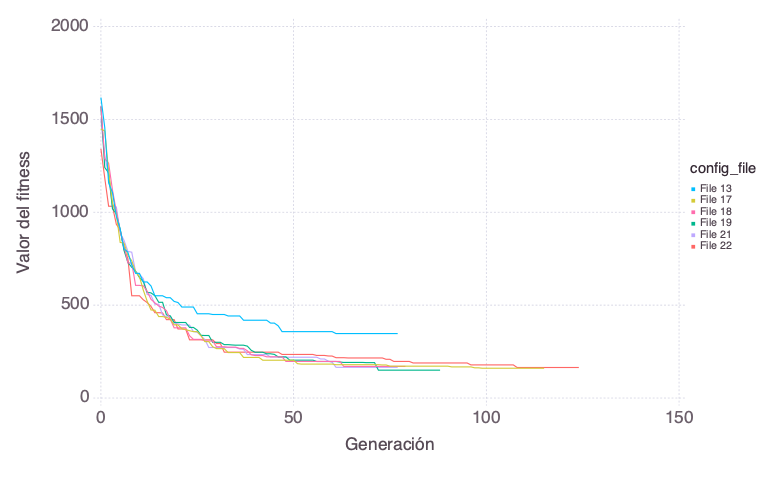
\includegraphics[scale=0.5]{../data/Plots/mutation_rate_executions.png}
	\caption{ Variación del valor del fitness a lo largo de las generaciones para los ficheros con mejor valor para cada fichero de configuración, variando la tasa de mutación}
    \label{fig:tasa_mutacion_variacion_generacion}
\end{figure}

Para explorar el comportamiento del algoritmo al cambiar la tasa de mutación se han usado los ficheros del 15 al 23, ver presentes en el Anexo \ref{subsect:config_file}. En la
Tabla \ref{tab:exploracion_tasa_mutacion} solo se han añadido los que presentan diferencia con la configuración 13. En esta tabla se puede ver que cambiando la tasa de mutación
de las castas se obtienen valores objetivamente mejores. Por ejemplo, el caso de la configuración 19 [\ref{subsect:config_file_19}], a pesar de tener la mayor desviación estándar,
es decir, teniendo la mayor dispersión de valores, es la que tiene mejor mediana de valor de la función del fitness. En la Figura \ref{fig:tasa_mutacion_variacion_generacion} se puede 
ver como los ficheros en los que se ha cambiado las tasas de mutación, además de durar más generaciones debido a que mantiene la diversidad durante más tiempo, obtiene
valores más pequeños de fitness.


\begin{table}[]
    \centering
    \begin{tabular}{|c|c|c|c|c|c|}
    \hline
    \textbf{Config.} & \textbf{\begin{tabular}[c]{@{}c@{}}Tasa\\ de\\ mutación\end{tabular}}                                & \textbf{\begin{tabular}[c]{@{}c@{}}Mediana \\ mejor valor \\ de fitness\end{tabular}} & \textbf{\begin{tabular}[c]{@{}c@{}}Mediana \\ \# ejecuciones \\ de f\end{tabular}} & \textbf{\begin{tabular}[c]{@{}c@{}}$\sigma$\\ mejor valor\\ de fitness\end{tabular}} & \textbf{\begin{tabular}[c]{@{}c@{}}$\sigma$\\ \# ejecuciones \\ de f\end{tabular}} \\ \hline
    13 [\ref{subsect:config_file_13}]  & \begin{tabular}[c]{@{}c@{}}ALFA:10\\ BETA: 10\\ GAMMA: 10\\ DELTA: 10\\ EPSILON: 10\end{tabular}     & 367.07                                                                                & 512473.0                                                                           & 23.38                                                                         & 124996.18                                                                   \\ \hline
    17 [\ref{subsect:config_file_17}]  & \begin{tabular}[c]{@{}c@{}}ALFA: 5\\ BETA: 10\\ GAMMA: 15\\ DELTA: 20\\ EPSILON: 25\end{tabular}     & 174.16                                                                                & 666019.0                                                                           & 17.27                                                                         & 139365.89                                                                   \\ \hline
    18 [\ref{subsect:config_file_18}]  & \begin{tabular}[c]{@{}c@{}}ALFA: 5\\ BETA: 10\\ GAMMA: 20\\ DELTA: 25\\ EPSILON: 30\end{tabular}     & 193.71                                                                                & 648559.0                                                                           & 15.20                                                                         & 78935.72                                                                    \\ \hline
    19 [\ref{subsect:config_file_19}]  & \begin{tabular}[c]{@{}c@{}}ALFA: 5\\ BETA: 10\\ GAMMA: 25\\ DELTA: 30\\ EPSILON: 40\end{tabular}     & 186.31                                                                                & 655014.0                                                                           & 26.32                                                                         & 116351.11                                                                   \\ \hline
    21 [\ref{subsect:config_file_20}]  & \begin{tabular}[c]{@{}c@{}}ALFA: 5\\ BETA: 10\\ GAMMA: 30\\ DELTA: 35\\ EPSILON: 45\end{tabular}     & 211.39                                                                                & 639449.0                                                                           & 21.16                                                                         & 144132.16                                                                   \\ \hline
    22 [\ref{subsect:config_file_21}]  & \begin{tabular}[c]{@{}c@{}}ALFA: 5\\ BETA: 10\\ GAMMA: 30\\ DELTA: 40\\ EPSILON: 50\end{tabular}     & 190.76                                                                                & 646056.0                                                                           & 22.19                                                                         & 120232.35                                                                   \\ \hline
    \end{tabular}
    \caption{Resultados exploración del tamaño del cromosoma, variando la tasa de mutación}
    \label{tab:exploracion_tasa_mutacion}
\end{table}



	% Conclusiones
	\chapter{Conclusiones y trabajo futuro}

Al principio de este trabajo se definieron 3 objetivos a alcanzar en el TFG. En esta sección
se analizarán para ver si se han llegado a completar. Además se comentarán cuáles serán
los siguientes pasos de este algoritmo.

\section{Conclusión}

El primer objetivo era mejorar la diversidad en problemas de optimización mediante la división de la población en castas.
En las primeras ejecuciones se veía cómo la mejora del valor de fitness empezaba a disminuir a partir de la generación 20. Sin embargo,
en las últimas ejecuciones, tras haber hecho la exploración de los parámetros, el algoritmo no se queda estancado en generaciones
tan tempranas. Para poder afirmar si mejora la diversidad habría que hacer una comparación más precisa con respecto al panorama actual 
de metaheurísticas. Pero para este objetivo, se puede concluir que con una buena elección de los parámetros iniciales se 
puede llegar a mantener una población más diversa que un algoritmo genético con los operadores básicos.

El segundo objetivo era desarrollar una herramienta de altas prestaciones para la ejecución de algoritmos evolutivos. En comparación
con la primera versión del algoritmo desarrollada en Python, se puede confirmar que esta versión es mucho más rápida. En Python tardaba alrededor
de horas en ejecutarse, mientras que en esta nueva versión en Julia no se llega al minuto. 

El tercer objetivo era aplicar el desarrollo ágil en la ciencia. Durante todo el trabajo se ha tenido una mentalidad ágil, preparada para adaptarse ante 
cualquier cambio de planificación, desarrollando en iteraciones que aportaban valor inmediato al producto.

\section{Trabajo futuro}

En un futuro sería interesante comprobar cómo se comporta el algoritmo al aplicarle paralelismo o investigar la comunicación entre las castas. 

Este trabajo ha sido presentado en ``International Seminar on Computational Intelligence 2021 (ISCI'21)``. Además será publicado 
en la recopilación de papers de este seminario.

	% Trabajos futuros
	\chapter{Anexos}

\section{Ficheros de configuración} \label{subsect:config_file}

\subsection{Fichero de configuración 1} \label{subsect:config_file_1}

\begin{lstlisting}[
    basicstyle=\small
]
{
    "CHROMOSOME_SIZE": 2,
    "POPULATION_SIZE": 100,
    "MAX_GENERATIONS": 15,
    "POPULATION_PERCENTAGE": {
        "ALPHA": 10,
        "BETA": 20,
        "GAMMA": 20,
        "DELTA": 20,
        "EPSILON": 30
    },
    "MUTATION_RATE": {
        "ALPHA": 10,
        "BETA": 10,
        "GAMMA": 10,
        "DELTA": 10,
        "EPSILON": 10
    }
}

\end{lstlisting}

\subsection{Fichero de configuración 2} \label{subsect:config_file_2}

\begin{lstlisting}[
    basicstyle=\small
]
{
    "CHROMOSOME_SIZE": 3,
    "POPULATION_SIZE": 100,
    "MAX_GENERATIONS": 15,
    "POPULATION_PERCENTAGE": {
        "ALPHA": 10,
        "BETA": 20,
        "GAMMA": 20,
        "DELTA": 20,
        "EPSILON": 30
    },
    "MUTATION_RATE": {
        "ALPHA": 10,
        "BETA": 10,
        "GAMMA": 10,
        "DELTA": 10,
        "EPSILON": 10
    }
}
   
\end{lstlisting}

\subsection{Fichero de configuración 3} \label{subsect:config_file_3}

\begin{lstlisting}[
    basicstyle=\small
]
{
    "CHROMOSOME_SIZE": 5,
    "POPULATION_SIZE": 100,
    "MAX_GENERATIONS": 15,
    "POPULATION_PERCENTAGE": {
        "ALPHA": 10,
        "BETA": 20,
        "GAMMA": 20,
        "DELTA": 20,
        "EPSILON": 30
    },
    "MUTATION_RATE": {
        "ALPHA": 10,
        "BETA": 10,
        "GAMMA": 10,
        "DELTA": 10,
        "EPSILON": 10
    }
}
   
\end{lstlisting}

\subsection{Fichero de configuración 4} \label{subsect:config_file_4}
\begin{lstlisting}[
    basicstyle=\small
]
{
    "CHROMOSOME_SIZE": 10,
    "POPULATION_SIZE": 100,
    "MAX_GENERATIONS": 15,
    "POPULATION_PERCENTAGE": {
        "ALPHA": 10,
        "BETA": 20,
        "GAMMA": 20,
        "DELTA": 20,
        "EPSILON": 30
    },
    "MUTATION_RATE": {
        "ALPHA": 10,
        "BETA": 10,
        "GAMMA": 10,
        "DELTA": 10,
        "EPSILON": 10
    }
}
   
\end{lstlisting}

\subsection{Fichero de configuración 5} \label{subsect:config_file_5}

\begin{lstlisting}[
    basicstyle=\small
]
{
    "CHROMOSOME_SIZE": 20,
    "POPULATION_SIZE": 100,
    "MAX_GENERATIONS": 15,
    "POPULATION_PERCENTAGE": {
        "ALPHA": 10,
        "BETA": 20,
        "GAMMA": 20,
        "DELTA": 20,
        "EPSILON": 30
    },
    "MUTATION_RATE": {
        "ALPHA": 10,
        "BETA": 10,
        "GAMMA": 10,
        "DELTA": 10,
        "EPSILON": 10
    }
}
   
\end{lstlisting}

\subsection{Fichero de configuración 6} \label{subsect:config_file_6}

\begin{lstlisting}[
    basicstyle=\small
]
{
    "CHROMOSOME_SIZE": 40,
    "POPULATION_SIZE": 100,
    "MAX_GENERATIONS": 15,
    "POPULATION_PERCENTAGE": {
        "ALPHA": 10,
        "BETA": 20,
        "GAMMA": 20,
        "DELTA": 20,
        "EPSILON": 30
    },
    "MUTATION_RATE": {
        "ALPHA": 10,
        "BETA": 10,
        "GAMMA": 10,
        "DELTA": 10,
        "EPSILON": 10
    }
}
   
\end{lstlisting}

\subsection{Fichero de configuración 7} \label{subsect:config_file_7}

\begin{lstlisting}[
    basicstyle=\small
]
{
    "CHROMOSOME_SIZE": 10,
    "POPULATION_SIZE": 150,
    "MAX_GENERATIONS": 15,
    "POPULATION_PERCENTAGE": {
        "ALPHA": 10,
        "BETA": 20,
        "GAMMA": 20,
        "DELTA": 20,
        "EPSILON": 30
    },
    "MUTATION_RATE": {
        "ALPHA": 10,
        "BETA": 10,
        "GAMMA": 10,
        "DELTA": 10,
        "EPSILON": 10
    }
}
   
\end{lstlisting}

\subsection{Fichero de configuración 8} \label{subsect:config_file_8}

\begin{lstlisting}[
    basicstyle=\small
]
{
    "CHROMOSOME_SIZE": 10,
    "POPULATION_SIZE": 300,
    "MAX_GENERATIONS": 15,
    "POPULATION_PERCENTAGE": {
        "ALPHA": 10,
        "BETA": 20,
        "GAMMA": 20,
        "DELTA": 20,
        "EPSILON": 30
    },
    "MUTATION_RATE": {
        "ALPHA": 10,
        "BETA": 10,
        "GAMMA": 10,
        "DELTA": 10,
        "EPSILON": 10
    }
}
   
\end{lstlisting}

\subsection{Fichero de configuración 9} \label{subsect:config_file_9}

\begin{lstlisting}[
    basicstyle=\small
]
{
    "CHROMOSOME_SIZE": 10,
    "POPULATION_SIZE": 500,
    "MAX_GENERATIONS": 15,
    "POPULATION_PERCENTAGE": {
        "ALPHA": 10,
        "BETA": 20,
        "GAMMA": 20,
        "DELTA": 20,
        "EPSILON": 30
    },
    "MUTATION_RATE": {
        "ALPHA": 10,
        "BETA": 10,
        "GAMMA": 10,
        "DELTA": 10,
        "EPSILON": 10
    }
}
   
\end{lstlisting}

\subsection{Fichero de configuración 10} \label{subsect:config_file_10}

\begin{lstlisting}[
    basicstyle=\small
]
{
    "CHROMOSOME_SIZE": 10,
    "POPULATION_SIZE": 1000,
    "MAX_GENERATIONS": 15,
    "POPULATION_PERCENTAGE": {
        "ALPHA": 10,
        "BETA": 20,
        "GAMMA": 20,
        "DELTA": 20,
        "EPSILON": 30
    },
    "MUTATION_RATE": {
        "ALPHA": 10,
        "BETA": 10,
        "GAMMA": 10,
        "DELTA": 10,
        "EPSILON": 10
    }
}
   
\end{lstlisting}

\subsection{Fichero de configuración 11} \label{subsect:config_file_11}

\begin{lstlisting}[
    basicstyle=\small
]
{
    "CHROMOSOME_SIZE": 15,
    "POPULATION_SIZE": 1500,
    "MAX_GENERATIONS": 15,
    "POPULATION_PERCENTAGE": {
        "ALPHA": 10,
        "BETA": 20,
        "GAMMA": 20,
        "DELTA": 20,
        "EPSILON": 30
    },
    "MUTATION_RATE": {
        "ALPHA": 10,
        "BETA": 10,
        "GAMMA": 10,
        "DELTA": 10,
        "EPSILON": 10
    }
}
   
\end{lstlisting}

\subsection{Fichero de configuración 12} \label{subsect:config_file_12}

\begin{lstlisting}[
    basicstyle=\small
]
{
    "CHROMOSOME_SIZE": 30,
    "POPULATION_SIZE": 3000,
    "MAX_GENERATIONS": 15,
    "POPULATION_PERCENTAGE": {
        "ALPHA": 10,
        "BETA": 20,
        "GAMMA": 20,
        "DELTA": 20,
        "EPSILON": 30
    },
    "MUTATION_RATE": {
        "ALPHA": 10,
        "BETA": 10,
        "GAMMA": 10,
        "DELTA": 10,
        "EPSILON": 10
    }
}
   
\end{lstlisting}

\subsection{Fichero de configuración 13} \label{subsect:config_file_13}

\begin{lstlisting}[
    basicstyle=\small
]
{
    "CHROMOSOME_SIZE": 50,
    "POPULATION_SIZE": 5000,
    "MAX_GENERATIONS": 15,
    "POPULATION_PERCENTAGE": {
        "ALPHA": 10,
        "BETA": 20,
        "GAMMA": 20,
        "DELTA": 20,
        "EPSILON": 30
    },
    "MUTATION_RATE": {
        "ALPHA": 10,
        "BETA": 10,
        "GAMMA": 10,
        "DELTA": 10,
        "EPSILON": 10
    }
}
   
\end{lstlisting}

\subsection{Fichero de configuración 14} \label{subsect:config_file_14}

\begin{lstlisting}[
    basicstyle=\small
]
{
    "CHROMOSOME_SIZE": 100,
    "POPULATION_SIZE": 10000,
    "MAX_GENERATIONS": 15,
    "POPULATION_PERCENTAGE": {
        "ALPHA": 10,
        "BETA": 20,
        "GAMMA": 20,
        "DELTA": 20,
        "EPSILON": 30
    },
    "MUTATION_RATE": {
        "ALPHA": 10,
        "BETA": 10,
        "GAMMA": 10,
        "DELTA": 10,
        "EPSILON": 10
    }
}
   
\end{lstlisting}


\subsection{Fichero de configuración 15} \label{subsect:config_file_15}

\begin{lstlisting}[
    basicstyle=\small
]
{
    "CHROMOSOME_SIZE": 50,
    "POPULATION_SIZE": 10000,
    "MAX_GENERATIONS": 15,
    "POPULATION_PERCENTAGE": {
        "ALPHA": 10,
        "BETA": 20,
        "GAMMA": 20,
        "DELTA": 20,
        "EPSILON": 30
    },
    "MUTATION_RATE": {
        "ALPHA": 10,
        "BETA": 20,
        "GAMMA": 30,
        "DELTA": 40,
        "EPSILON": 50
    }
}
   
\end{lstlisting}

\subsection{Fichero de configuración 16} \label{subsect:config_file_16}

\begin{lstlisting}[
    basicstyle=\small
]
{
    "CHROMOSOME_SIZE": 50,
    "POPULATION_SIZE": 5000,
    "MAX_GENERATIONS": 15,
    "POPULATION_PERCENTAGE": {
        "ALPHA": 10,
        "BETA": 20,
        "GAMMA": 20,
        "DELTA": 20,
        "EPSILON": 30
    },
    "MUTATION_RATE": {
        "ALPHA": 10,
        "BETA": 15,
        "GAMMA": 20,
        "DELTA": 25,
        "EPSILON": 30
    }
}
   
\end{lstlisting}

\subsection{Fichero de configuración 17} \label{subsect:config_file_17}

\begin{lstlisting}[
    basicstyle=\small
]
{
    "CHROMOSOME_SIZE": 50,
    "POPULATION_SIZE": 5000,
    "MAX_GENERATIONS": 15,
    "POPULATION_PERCENTAGE": {
        "ALPHA": 10,
        "BETA": 20,
        "GAMMA": 20,
        "DELTA": 20,
        "EPSILON": 30
    },
    "MUTATION_RATE": {
        "ALPHA": 5,
        "BETA": 10,
        "GAMMA": 15,
        "DELTA": 20,
        "EPSILON": 25
    }
}
   
\end{lstlisting}

\subsection{Fichero de configuración 18} \label{subsect:config_file_18}

\begin{lstlisting}[
    basicstyle=\small
]
{
    "CHROMOSOME_SIZE": 50,
    "POPULATION_SIZE": 5000,
    "MAX_GENERATIONS": 15,
    "POPULATION_PERCENTAGE": {
        "ALPHA": 10,
        "BETA": 20,
        "GAMMA": 20,
        "DELTA": 20,
        "EPSILON": 30
    },
    "MUTATION_RATE": {
        "ALPHA": 5,
        "BETA": 10,
        "GAMMA": 20,
        "DELTA": 25,
        "EPSILON": 30
    }
}
   
\end{lstlisting}

\subsection{Fichero de configuración 19} \label{subsect:config_file_19}

\begin{lstlisting}[
    basicstyle=\small
]
{
    "CHROMOSOME_SIZE": 50,
    "POPULATION_SIZE": 5000,
    "MAX_GENERATIONS": 15,
    "POPULATION_PERCENTAGE": {
        "ALPHA": 10,
        "BETA": 20,
        "GAMMA": 20,
        "DELTA": 20,
        "EPSILON": 30
    },
    "MUTATION_RATE": {
        "ALPHA": 5,
        "BETA": 10,
        "GAMMA": 25,
        "DELTA": 30,
        "EPSILON": 40
    }
}
   
\end{lstlisting}

\subsection{Fichero de configuración 20} \label{subsect:config_file_20}

\begin{lstlisting}[
    basicstyle=\small
]
{
    "CHROMOSOME_SIZE": 50,
    "POPULATION_SIZE": 5000,
    "MAX_GENERATIONS": 15,
    "POPULATION_PERCENTAGE": {
        "ALPHA": 10,
        "BETA": 20,
        "GAMMA": 20,
        "DELTA": 20,
        "EPSILON": 30
    },
    "MUTATION_RATE": {
        "ALPHA": 10,
        "BETA": 15,
        "GAMMA": 25,
        "DELTA": 30,
        "EPSILON": 40
    }
}
\end{lstlisting}

\subsection{Fichero de configuración 21} \label{subsect:config_file_21}

\begin{lstlisting}[
    basicstyle=\small
]
{
    "CHROMOSOME_SIZE": 50,
    "POPULATION_SIZE": 5000,
    "MAX_GENERATIONS": 15,
    "POPULATION_PERCENTAGE": {
        "ALPHA": 10,
        "BETA": 20,
        "GAMMA": 20,
        "DELTA": 20,
        "EPSILON": 30
    },
    "MUTATION_RATE": {
        "ALPHA": 5,
        "BETA": 10,
        "GAMMA": 30,
        "DELTA": 35,
        "EPSILON": 45
    }
}
\end{lstlisting}

\subsection{Fichero de configuración 22} \label{subsect:config_file_22}

\begin{lstlisting}[
    basicstyle=\small
]
{
    "CHROMOSOME_SIZE": 50,
    "POPULATION_SIZE": 5000,
    "MAX_GENERATIONS": 15,
    "POPULATION_PERCENTAGE": {
        "ALPHA": 10,
        "BETA": 20,
        "GAMMA": 20,
        "DELTA": 20,
        "EPSILON": 30
    },
    "MUTATION_RATE": {
        "ALPHA": 5,
        "BETA": 10,
        "GAMMA": 30,
        "DELTA": 40,
        "EPSILON": 50
    }
}  
\end{lstlisting}

\subsection{Fichero de configuración 23} \label{subsect:config_file_23}

\begin{lstlisting}[
    basicstyle=\small
]
{
    "CHROMOSOME_SIZE": 50,
    "POPULATION_SIZE": 5000,
    "MAX_GENERATIONS": 15,
    "POPULATION_PERCENTAGE": {
        "ALPHA": 10,
        "BETA": 20,
        "GAMMA": 20,
        "DELTA": 20,
        "EPSILON": 30
    },
    "MUTATION_RATE": {
        "ALPHA": 5,
        "BETA": 10,
        "GAMMA": 30,
        "DELTA": 40,
        "EPSILON": 50
    }
}
   
\end{lstlisting}

	\newpage
	\bibliography{bibliografia}
	\bibliographystyle{plain}
	
\end{document}

